\documentclass[a0paper,portrait]{baposter}

\usepackage{relsize}		% For \smaller
\usepackage{url}			% For \url
% \usepackage{epstopdf}	% Included EPS files automatically converted to PDF to include with pdflatex

%%% Global Settings %%%%%%%%%%%%%%%%%%%%%%%%%%%%%%%%%%%%%%%%%%%%%%%%%%%%%%%%%%%

\graphicspath{{images/}}	% Root directory of the pictures
% \tracingstats=2			% Enabled LaTeX logging with conditionals

%%% Color Definitions %%%%%%%%%%%%%%%%%%%%%%%%%%%%%%%%%%%%%%%%%%%%%%%%%%%%%%%%%

\definecolor{bordercol}{RGB}{40,40,40}
\definecolor{headercol1}{RGB}{186,215,230}
\definecolor{headercol2}{RGB}{80,80,80}
\definecolor{headerfontcol}{RGB}{0,0,0}
\definecolor{boxcolor}{RGB}{186,215,230}

%%%%%%%%%%%%%%%%%%%%%%%%%%%%%%%%%%%%%%%%%%%%%%%%%%%%%%%%%%%%%%%%%%%%%%%%%%%%%%%%
%%% Utility functions %%%%%%%%%%%%%%%%%%%%%%%%%%%%%%%%%%%%%%%%%%%%%%%%%%%%%%%%%%

%%% Save space in lists. Use this after the opening of the list %%%%%%%%%%%%%%%%
\newcommand{\compresslist}{
	\setlength{\itemsep}{1pt}
	\setlength{\parskip}{0pt}
	\setlength{\parsep}{0pt}
}

%%%%%%%%%%%%%%%%%%%%%%%%%%%%%%%%%%%%%%%%%%%%%%%%%%%%%%%%%%%%%%%%%%%%%%%%%%%%%%%
%%% Document Start %%%%%%%%%%%%%%%%%%%%%%%%%%%%%%%%%%%%%%%%%%%%%%%%%%%%%%%%%%%%
%%%%%%%%%%%%%%%%%%%%%%%%%%%%%%%%%%%%%%%%%%%%%%%%%%%%%%%%%%%%%%%%%%%%%%%%%%%%%%%

\begin{document}
%%% Setting Background Image %%%%%%%%%%%%%%%%%%%%%%%%%%%%%%%%%%%%%%%%%%%%%%%%%%
\background{
	\begin{tikzpicture}[remember picture,overlay]%
	\draw (current page.north west)+(-2em,2em) node[anchor=north west]
	{
\includegraphics[height=1.1\textheight]{background}};
	\end{tikzpicture}
}

%%% General Poster Settings %%%%%%%%%%%%%%%%%%%%%%%%%%%%%%%%%%%%%%%%%%%%%%%%%%%
%%%%%% Eye Catcher, Title, Authors and University Images %%%%%%%%%%%%%%%%%%%%%%
\begin{poster}{
	grid=false,
	% Option is left on true though the eyecatcher is not used. The reason is
	% that we have a bit nicer looking title and author formatting in the headercol
	% this way
	%eyecatcher=false,
	borderColor=bordercol,
	headerColorOne=headercol1,
	headerColorTwo=headercol2,
	headerFontColor=headerfontcol,
	% Only simple background color used, no shading, so boxColorTwo isn't necessary
	boxColorOne=boxcolor,
	headershape=roundedright,
	headerfont=\Large\sf\bf,
	textborder=rectangle,
	background=user,
	headerborder=open,
  boxshade=plain
}
%%% Eye Cacther %%%%%%%%%%%%%%%%%%%%%%%%%%%%%%%%%%%%%%%%%%%%%%%%%%%%%%%%%%%%%%%
{
	Eye Catcher, empty if option eyecatcher=false - unused
}
%%% Title %%%%%%%%%%%%%%%%%%%%%%%%%%%%%%%%%%%%%%%%%%%%%%%%%%%%%%%%%%%%%%%%%%%%%
{\sf\bf
	Automation of Monitoring of Road Surface Conditions Using Drivers' Mobile Devices
}
%%% Authors %%%%%%%%%%%%%%%%%%%%%%%%%%%%%%%%%%%%%%%%%%%%%%%%%%%%%%%%%%%%%%%%%%%
{
	\vspace{1em} Nikita Kulakov, Ivan Loginov\\
	{\smaller 312563@niuitmo.ru, ivan.loginov@niutmo.ru}
}
%%% Logo %%%%%%%%%%%%%%%%%%%%%%%%%%%%%%%%%%%%%%%%%%%%%%%%%%%%%%%%%%%%%%%%%%%%%%
{
% The logos are compressed a bit into a simple box to make them smaller on the result
% (Wasn't able to find any bigger of them.)
\setlength\fboxsep{0pt}
\setlength\fboxrule{0.5pt}
	\fbox{
		\begin{minipage}{14em}
			
\includegraphics[width=10em,height=4em]{logo_osnovnoy_russkiy_chernyy}
			
\includegraphics[width=4em,height=4em]{itmo-duck-large-black-bg}
		\end{minipage}
	}
}

\headerbox{Problem}{name=problem,column=0,row=0}{
The problem of road quality is important: poor roads increase the likelihood of traffic accidents, increase the cost of maintaining vehicles and driving time. In addition, untimely repairs increase the cost of maintaining road sections. As a result of our work, a solution for monitoring the condition of the road surface was proposed.
}

\headerbox{Basic Idea}{name=idea,column=0,below=problem}{
The system uses mobile phones to collect raw sensor data from the accelerometer, gyroscope, and GPS, which is transmitted via MQTT to backend services without any local processing. This design preserves battery life and avoids taxing the device’s CPU, enabling seamless integration as an independent module within existing navigation or map applications. On the server side, the data undergoes interpolation and aggregation. The high volume of user data compensates for the low quality or variability of individual sensors, allowing statistically reliable detection of road conditions and enhancing accuracy through collective measurement.

}

\headerbox{Models and Prediction}{name=models,column=0,below=idea}{
\textbf{M1 (Deterministic, no preprocessing):} Direct prediction on raw data. Score: 0.42. \\

\textbf{M2 (Deterministic, with preprocessing):} Noise reduction $\rightarrow$ Feature extraction $\rightarrow$ Feature selection ($k=24$) $\rightarrow$ Deterministic prediction. Score: 0.42. \\

\textbf{M3 (CART, no speed):} Preprocessing as in M2 $\rightarrow$ \texttt{DecisionTreeRegressor}, params: criterion=\texttt{squared\_error}, depth=5. \\

\textbf{M4 (Random Forest, no speed):} Preprocessing as in M2 $\rightarrow$ \texttt{RandomForestRegressor}, params: n=100, depth=3. \\

\textbf{M5 (XGBoost, no speed):} Preprocessing as in M2 $\rightarrow$ \texttt{XGBRegressor}, params: obj=\texttt{reg:squarederror}, lr=0.3, depth=6. \\

\textbf{M6 (XGBoost, with speed):} Same as M5 with speed as additional feature. \\

In addition, a data preprocessing algorithm was implemented on the backend, including interpolation, filtering, and Fourier transform, to further improve the accuracy of predictive models.
}

\headerbox{References}{name=references,column=0,below=models,above=bottom}{
\smaller													% Make the whole text smaller
\vspace{-0.4em} 										% Save some space at the beginning
\bibliographystyle{plain}							% Use plain style
\renewcommand{\section}[2]{\vskip 0.05em}		% Omit "References" title
\begin{thebibliography}{1}							% Simple bibliography with widest label of 1
\itemsep=-0.01em										% Save space between the separation
\setlength{\baselineskip}{0.4em}					% Save space with longer lines
\bibitem{road-1} Ekaterina Aleksandrovna Ponomareva, Aleksandra Dmitrievna Savina Factors influencing mortality in road accidents // Economic policy. 2022. No. 4. URL: https://cyberleninka.ru/article/n/faktory-vliyayuschie-na-smertnost-v-dtp.
\bibitem{road-2} Shabazov M.M. Influence Of Road Quality On The Cost Of Cargo Transportation And On Fuel Consumption // World Science. 2023. No. 5 (74). URL: https://cyberleninka.ru/article/n/vliyanie-kachestva-dorog-na-stoimost-perevozki-gruzov-i-na- rashod-topliva.
\bibitem{menegazzo-road-surface}J. Menegazzo and A. von Wangenheim, "Multi-Contextual and Multi-Aspect Analysis for Road Surface Type Classification Through Inertial Sensors and Deep Learning," 2020 X Brazilian Symposium on Computing Systems Engineering (SBESC), Florianopolis, 2020, pp. 1-8, doi: 10.1109/SBESC51047.2020.9277846.0)
\end{thebibliography}
}

\headerbox{System Architecture}{name=architecture,span=2,column=1,row=0}{
  This system architecture depicts a data processing pipeline where a \textbf{mobile application} sends monitoring data via MQTT to a \textbf{Kafka MQTT Proxy}, which forwards the data to a \textbf{Kafka cluster (Kafka KRaft)} under the \textbf{topic monitoring}. A forecasting service consumes this topic, performs computations, and produces results to the \textbf{topic points}. A result processing service then consumes from points and inserts data into a \textbf{ClickHouse database}. \textbf{User queries} are handled through a dedicated service that performs SQL queries on \textbf{ClickHouse database} to retrieve stored aggregated results.

\vspace{0.4em}

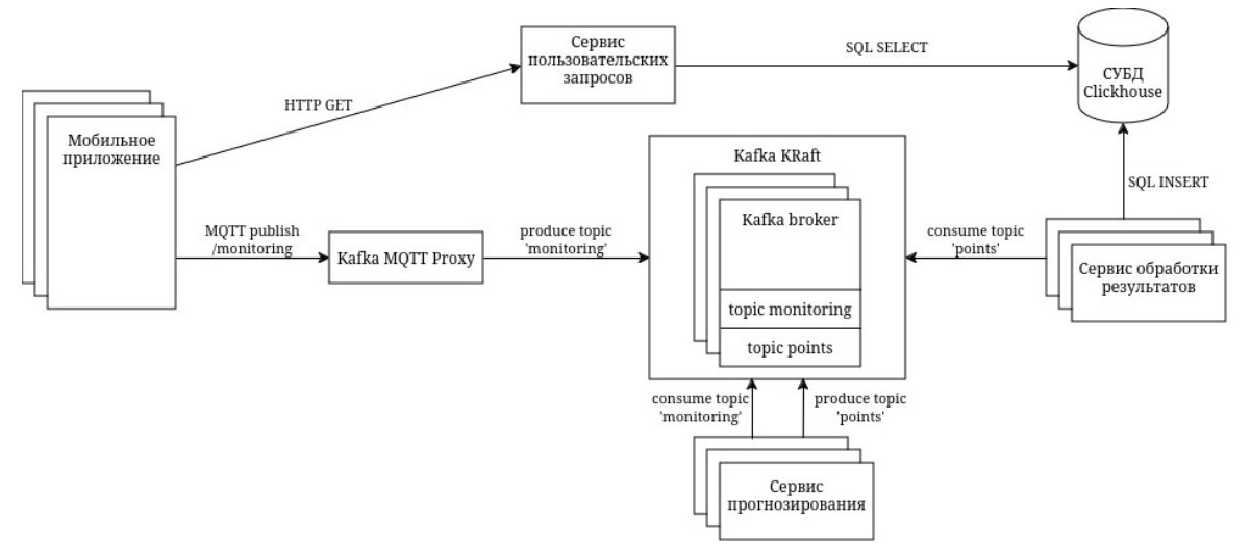
\includegraphics[width=\linewidth]{basic_architecture}

\vspace{-0.2em}
}

\headerbox{Testing and Overview}{name=testing,span=2,column=1,below=architecture,above=bottom}{
  Results are extremely dependant on trained models and accuracy of mobile phone devices (accelerometer, gyroscope and GPS) or data volume. Testing on both real and training data demonstrated the feasibility of using the developed system to achieve the intended goal. On a server with 2 cores (2.6 GHz) and 4 GB of RAM, the system processed 4,200 user messages—each containing 30 seconds of sensor data—in 150 seconds. The best-performing model on real data, an XGBoost model excluding the speed attribute, achieved a coefficient of determination (R²) of 0.70.

\vspace{-0.4em}
\begin{center}
	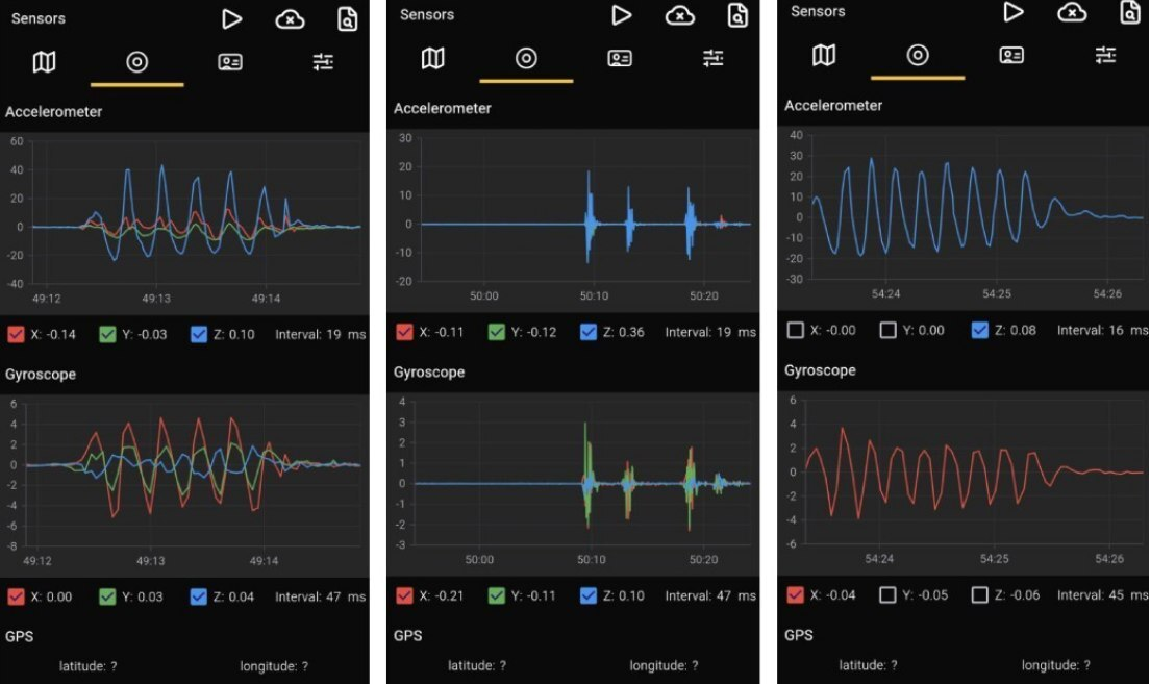
\includegraphics[width=\linewidth]{sensor_view}
\end{center}

\vspace{-0.4em}

The image displays monitoring results of road conditions across multiple map segments. Roads are color-coded from green (indicating good condition) to red (indicating poor condition), forming a gradient to reflect varying quality.

\vspace{-0.4em}
\begin{center}
	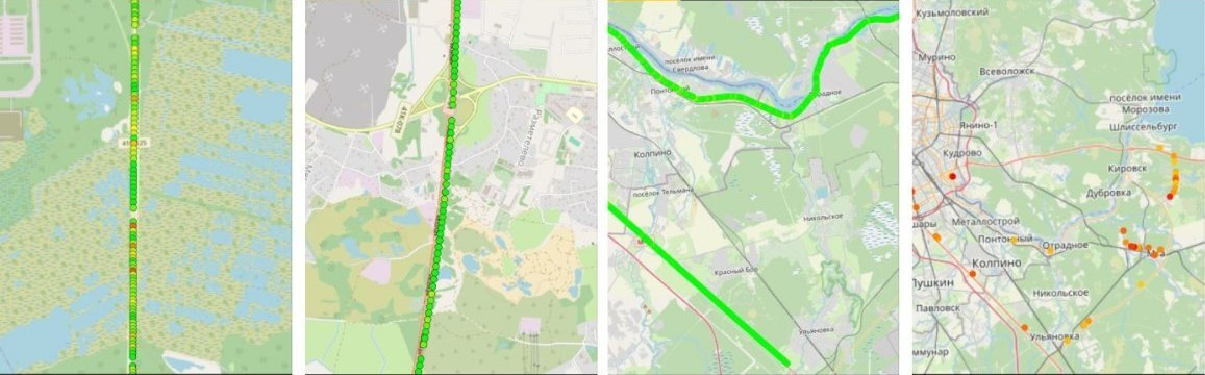
\includegraphics[width=\linewidth]{map_view}
\end{center}
}

\end{poster}
\end{document}
